  % kobe.Rnw --
%
% Author: laurence kell <lauriekell@gmail.com>

%\VignetteIndexEntry{kobe}
% Meta information - fill between {} and do not remove %
% \VignetteIndexEntry{An R Package for plotting Kobe advice}
% \VignetteDepends{ggplot2, reshape, plyr}
% \VignettePackage{kobe}
%\VignetteKeywords{tRFMO, R}


\documentclass[shortnames,nojss,article]{jss}

\usepackage{booktabs,flafter} %,thumbpdf}
%\usepackage[onehalfspacing]{setspace}
\usepackage{natbib} \bibliographystyle{plain}
\usepackage{graphicx, psfrag, Sweave}
\usepackage{enumerate}
\usepackage{hyperref}

%\newcommand{\code}[1]{\texttt{#1}}
%\newcommand{\proglang}[1]{\textsf{#1}}
%\newcommand{\pkg}[1]{{\fontseries{b}\selectfont #1}}

\author{Laurence Kell\\ICCAT}
\Plainauthor{Laurence Kell}

\title{\pkg{kobe}: \proglang{R} tools for Tuna Management Advice}
\Plaintitle{kobe: R tools for Tuna Management Advice}

\Abstract{
  Scientific advice within the tuna Regional Fisheries Management Organisations (tRFMOs) is based the common Kobe framework. 
  Advice summarises the probabilities of biomass being greater than and fishing mortality less than the levels that can support
  maximum sustainable yield (MSY) for a range of management options.  
  This requires  estimates of current status relative to reference points and projections for
  the different management options. The \texttt{kobe} package can read in results from a variety of stock assessment packages and 
  summarise them in the Kobe format. 
}

\Keywords{\proglang{R}, tuna, RFMO, advice, fisheries, stock assessment, management}
\Plainkeywords{R, tuna, RFMO, advice, fisheries, stock assessment, management}

\Address{
  Laurence Kell \\
  ICCAT Secretariat\\ 		
  C/Coraz\'{o}n de Mar\'{\i}a, 8. \\
  28002 Madrid\\
  Spain\\ 
  
  E-mail: \email{Laurie.Kell@iccat.int}
}

%% need no \usepackage{Sweave.sty}

%

\begin{document}
\Sconcordance{concordance:kobe.tex:kobe.Rnw:%
1 78 1 1 13 54 1 1 3 2 0 1 1 3 0 1 3 13 0 1 2 2 1 1 3 2 0 1 1 3 0 2 2 %
13 0 1 2 11 1 1 3 2 0 2 1 3 0 1 2 1 1 1 3 5 0 2 2 6 0 1 1 6 0 1 2 1 3 5 %
0 1 2 2 1 1 2 13 0 1 2 2 1 1 2 13 0 1 2 2 1 1 2 4 0 1 2 20 1 1 5 8 0 1 %
2 11 1 1 8 11 0 1 2 15 1 1 3 2 0 1 1 4 0 1 2 8 1 1 2 1 0 1 1 12 0 1 2 9 %
1 1 2 1 0 1 1 1 2 12 0 1 2 6 1 1 5 8 0 1 2 7 1 1 6 8 0 1 2 1 1 1 2 4 0 %
1 2 7 1 1 2 1 0 1 4 6 0 1 2 5 1 1 4 7 0 1 2 4 1 1 3 15 0 1 2 8 1 1 3 2 %
0 1 2 1 0 1 10 12 0 1 2 6 1 1 2 1 0 1 17 16 0 1 2 1 3 1 0 2 1 1 3 1 0 1 %
11 9 0 1 1 4 0 1 2 17 1 1 2 1 0 1 2 3 1 3 0 1 2 28 1}


%------ Frontmatter ------
\title{Kobe Plotting}
\author{Laurie Kell\footnote{ICCAT}}
\date{June 2012}
\maketitle

\tableofcontents

\section{Introduction}

Scientific Advice within the tuna Regional Fisheries Management Organisations (tRFMOs) is based on the
\href{http://www.tuna-org.org/Documents/TRFMO3/K3-REC_ENG.pdf}{Kobe advice framework.} 
Advice is based on ensuring that they is a low risk of fishing mortality exceeding $F_{MSY}$ and biomass falling below $B_{MSY}$. 
This requires the calculation of the probabilities of $F$ \textless  $F_{MSY}$ and $B$ \textgreater $B_{MSY}$ for current stock status and a 
range of management options, generally total allowable catches (TAC).  

This requires, a stock assessment, estimates of reference points and stock projections, which can be performed in a variety of
software packages. The \texttt{kobe} package reads in results from the different input and output file formats and summarises 
them in the Kobe advice format.

The package provides methods for creating data.frames holding time series of $F/F_{MSY}$ and $SSB/B_{MSY}$ and for summarising, 
plotting and tablulation using using using the \pkg{plyr}, \pkg{ggplot2} and \pkg{tabular} packages.


\section{Data}

Estimates of stock status and exploitation level relative to MSY reference points can be obtained from a variety of stock assessment 
methods based on a variety of assumptions. For example biomass dynamic models which provide estimates of total biomass and harvest rate or 
age based models which provide estimates of spawning stock biomass and fishing mortality.

The different stock assessment methods have mainly been implemented as executable programs with a variety of input and output files 
in text format.  This can make it difficult to summarise results across methods, evaluate the consequences of the different assumption 
and to formulate advice in a common framework. Therefore in the \pkg{kobe} there are methods to read text files into a 
data.frames summarising stock (biomass or SSB) and harvest (fishing mortality or harvest rate) by scenarios (e.g. assessment run), 
management option (e.g. TACs) used in projecions and replicates from bootstraps or Monte Carlo Markov Chain simulations.

Currently there are methods for reading in stock assessment text files for ASPIC, Adapt, SS3 and MFCL (i.e. \code{kobeAspic}, \code{kobe2box}, 
\code{kobeSS} and \code{kobeMFCL}). 

Here we demonstrate how to read in outputs from \code{ASPIC}.

\subsection{kobeAspic}

Results from \code{ASPIC} are written to files with extensions that identify their contents, i.e.
bootstrapped assessment results are found in \code{.bio} and projections based on these in \code{.prb} files. 
These is a \code{.prb} file for each TAC, so to use \code{kobeAspic} requires 
specifying a single \code{.bio} file, multiple \code{.prb} files and a directory where they are found. 

Reading in the bootstrapped assessment

\begin{Schunk}
\begin{Sinput}
> ### Results from ASPIC bootstrapped assessment
> bio   ="http://www.iccat.int/stocka/Models/ASPIC/albs/2011/run2/aspic.bio"
> assmt =kobeAspic(bio)
\end{Sinput}
\end{Schunk}
\begin{Schunk}
\begin{Sinput}
> head(assmt)
\end{Sinput}
\begin{Soutput}
  iter year    stock      harvest     bmsy      fmsy
1    1 1956 1.800000 0.0004169473 110448.7 0.2479588
2    1 1957 1.873086 0.0139635494 110448.7 0.2479588
3    1 1958 1.915449 0.0198786446 110448.7 0.2479588
4    1 1959 1.940032 0.0891123383 110448.7 0.2479588
5    1 1960 1.928930 0.2009482466 110448.7 0.2479588
6    1 1961 1.880085 0.2110163113 110448.7 0.2479588
\end{Soutput}
\end{Schunk}

and a projection for a single TAC 

\begin{Schunk}
\begin{Sinput}
> ## Results from an ASPIC Projection
> prb  ="http://www.iccat.int/stocka/Models/ASPIC/albs/2011/run2/aspic_15000.prb"
> prj1 =kobeAspic(bio,prb)
\end{Sinput}
\end{Schunk}

\begin{Schunk}
\begin{Sinput}
> tail(prj1)
\end{Sinput}
\begin{Soutput}
      iter year     stock   harvest     bmsy      fmsy
71151  500 2020 0.7997950 0.7527672 206883.8 0.1173888
71161  500 2021 0.8408805 0.7162019 206883.8 0.1173888
71171  500 2022 0.8835242 0.6819915 206883.8 0.1173888
71181  500 2023 0.9273448 0.6502398 206883.8 0.1173888
71191  500 2024 0.9719148 0.6209882 206883.8 0.1173888
71201  500 2025 1.0167761 0.0000000 206883.8 0.1173888
\end{Soutput}
\end{Schunk}

By default \code{kobeAspic} returns all the simulations, however in addition four types of summary output can also be returned;  
these are specified by the \code{what} argument. As well as \code{sim} (the default of everthing), options are 
\code{trks} interquartiles and medians of stock and harvest;
\code{pts}  bootstrapped values in last year of assessment;
\code{smry} probability of being in kobe phase plot quadrants and
\code{wrms} randomly selected bootstrap runs.

If a single value is passed via \code{what} then a data.frame is returned, if more than one then list of data.frames is returned; useful 
when producing different plots and summaries.  

To read in the results from projections for a range of TACs first create a vector of files 
\begin{Schunk}
\begin{Sinput}
> ## Projections
> TACs=seq(15000,35000,5000)
> prb ="http://www.iccat.int/stocka/Models/ASPIC/albs/2011/run2/aspic_"
> prb =paste(prb,TACs,".prb",sep="")
\end{Sinput}
\end{Schunk}

In this case it is better to return subsets of the data for plotting
\begin{Schunk}
\begin{Sinput}
> ## Results
> prj=kobeAspic(bio,prb,what=c("pts","trks","smry"))
\end{Sinput}
\end{Schunk}

\begin{Schunk}
\begin{Sinput}
> class(prj)
\end{Sinput}
\begin{Soutput}
[1] "list"
\end{Soutput}
\begin{Sinput}
> names(prj)
\end{Sinput}
\begin{Soutput}
[1] "pts"  "trks" "smry"
\end{Soutput}
\end{Schunk}

\begin{Schunk}
\begin{Sinput}
> ## add TAC column to data.frame
> prj=llply(prj, transform, TAC=TACs[X1])
\end{Sinput}
\end{Schunk}

\code{pts} are the simulation results from the last year in the assessment;
\code{trks} summarise the time series by providing the medians and interquartiles. 
\begin{Schunk}
\begin{Sinput}
> head(prj$trks)
\end{Sinput}
\begin{Soutput}
  X1 year Percentile    stock      harvest   TAC
1  1 1956        75% 1.800002 0.0004401433 15000
2  1 1957        75% 1.899722 0.0148261963 15000
3  1 1958        75% 1.944386 0.0211279973 15000
4  1 1959        75% 1.963508 0.0944787954 15000
5  1 1960        75% 1.937559 0.2118392354 15000
6  1 1961        75% 1.879321 0.2214004342 15000
\end{Soutput}
\end{Schunk}

and \code{smry} provides the probabilities of being overfished or subject to overfishing.

\begin{Schunk}
\begin{Sinput}
> head(prj$smry)
\end{Sinput}
\begin{Soutput}
  X1 year    stock     harvest red yellow green overFished overFishing   TAC
1  1 1956 1.800000 0.000415844   0      0     1          0           0 15000
2  1 1957 1.873657 0.013922865   0      0     1          0           0 15000
3  1 1958 1.916143 0.019820714   0      0     1          0           0 15000
4  1 1959 1.940661 0.088869350   0      0     1          0           0 15000
5  1 1960 1.929268 0.200428382   0      0     1          0           0 15000
6  1 1961 1.875850 0.210521265   0      0     1          0           0 15000
\end{Soutput}
\end{Schunk}

There is also an example data set in \code{kobe} e.g.

\begin{Schunk}
\begin{Sinput}
> data(sims)
\end{Sinput}
\end{Schunk}

for use in the following examples


\section{Plotting}

\pkg{kobe} \href{http://ggplot2.org}{\code{ggplot2}} for plotting. This ia a plotting system for R, 
based on the grammar of graphics, which tries to take the good parts of base and lattice graphics and none of the bad parts. 
It takes care of many of  the fiddly details that make plotting a hassle (like drawing legends) as well as providing a powerful model 
of graphics that makes it easy to produce complex multi-layered graphics allowing the basic plots to be easily modified. 


\subsection{ggplot2}

There are two interfaces \code{qplot} e.g.

\code{qplot(x=year,y=stock,data=prj$wrms)}

or \code{ggplot2}  e.g.

\begin{figure}\begin{center}
\begin{Schunk}
\begin{Sinput}
> ggplot(assmt)                                       + 
+   geom_hline(aes(yintercept=1),col="red",size=2)    + 
+   geom_line( aes(year,stock,group=iter,col=iter))   +
+   theme(legend.position="none")
\end{Sinput}
\end{Schunk}
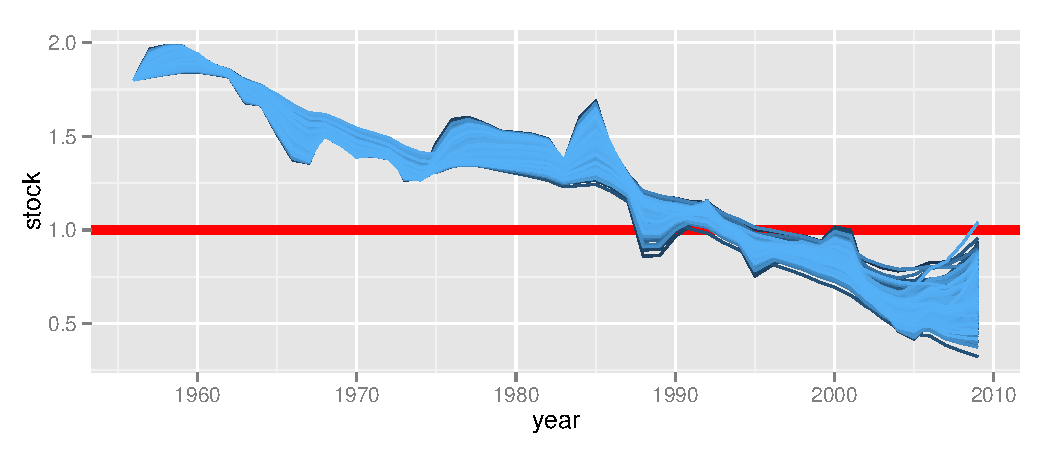
\includegraphics{kobe-013}
\caption{Plots of time series of biomass by bootstrap}
\end{center}\end{figure}

\clearpage

The syntax of \code{qplot} is similar to \code{plot} in base graphi	cs and so it is initially easier to use. 
While \code{ggplot} provides more flexibility, where as in the above example, extra elements can be added to the basic plots.

For example here we plot the historic and projected times series of biomass and harvest by TAC for the interquartiles and medians in
\code{trks}

\begin{figure}\begin{center}
\begin{Schunk}
\begin{Sinput}
> ### tracks
> ggplot(subset(prj$trks,year<=2020))                           +
+   geom_line(aes(year,stock,  linetype=Percentile),col="blue") +
+   geom_line(aes(year,harvest,linetype=Percentile),col= "red") +
+   scale_linetype_manual(values=c(2,1,2))                      +
+   coord_cartesian(ylim=c(0,3))                                +
+   facet_wrap(~TAC,ncol=2)
\end{Sinput}
\end{Schunk}
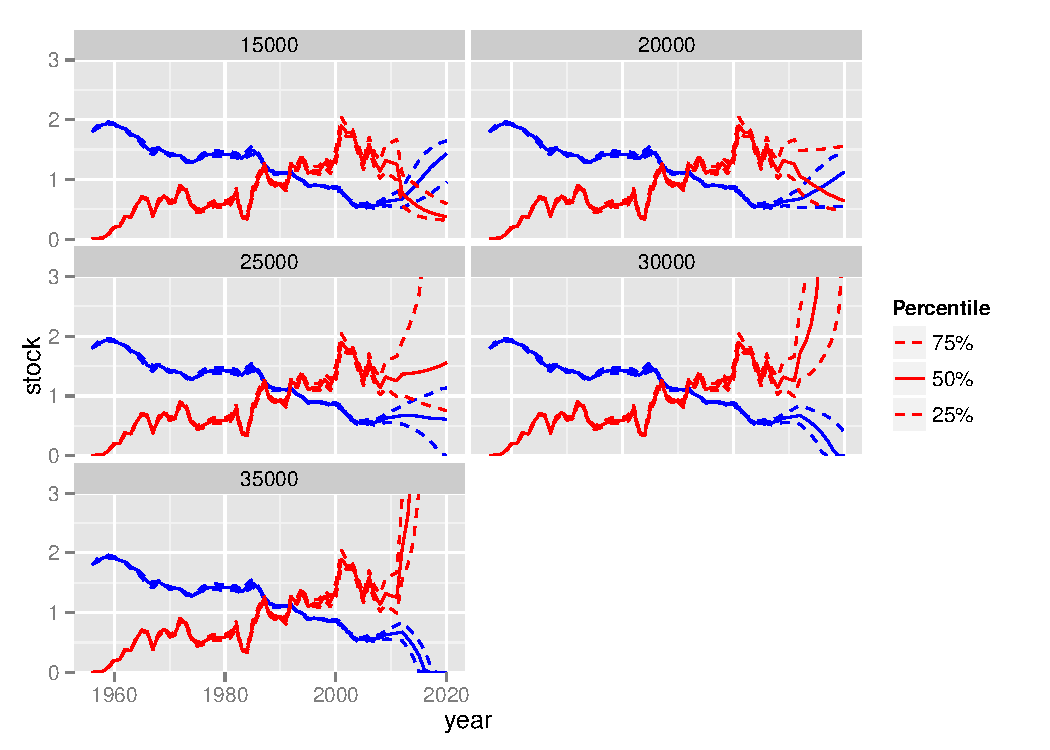
\includegraphics{kobe-014}
\caption{Historic and projected times series of biomass (blue) and harvest (red) by TAC for the interquartiles and medians}
\end{center}\end{figure}

\clearpage

\subsection{Kobe Framework}

The Kobe framework is based on a phase plot where $F : F_{MSY}$ is plotted against $Biomass : B_{MSY}$; quadrants are colour coded i.e.
green (not overfished, no overfishing), red quadrant (i.e. overfished and overfishing) or yellow (otherwise).
Since the main management objective is to keep a stock in the green quadrant projections are performed to evaluate the consequences of different TACs. 
The Kobe II strategy matrice (K2SM) summarise the probabilities for different levels of TAC across multiple years of being in the green quadrant.

\subsubsection{Phase Plot}

An example phase plot is shown in figure \ref{}
\begin{figure}\begin{center}
\begin{Schunk}
\begin{Sinput}
> kp=kobePhase(subset(sims, year==2010 & TAC==15000)) +
+          geom_point(aes(stock,harvest,group=Run,col=Run)) 
> kp
\end{Sinput}
\end{Schunk}
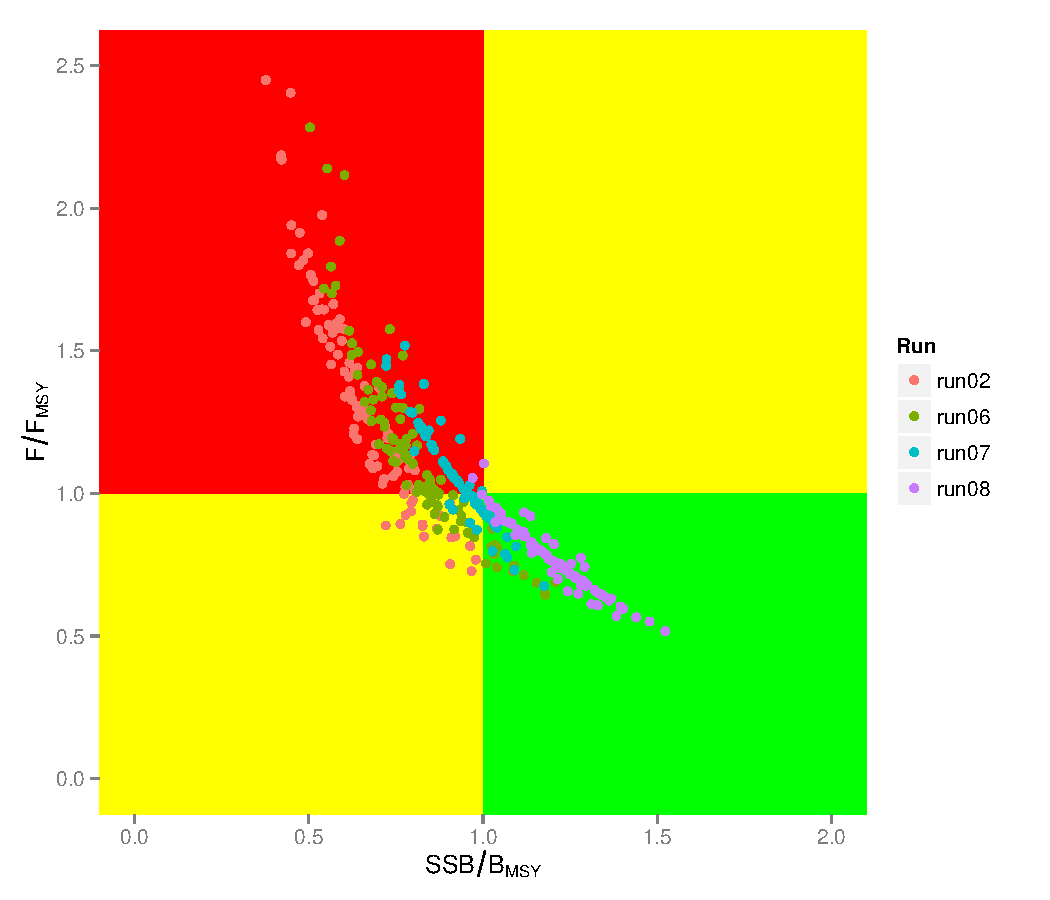
\includegraphics{kobe-015}
\caption{Phase plot of fishng mortality and stock status reletive to $F_{MSY}$ and  $B_{MSY}$}
\label{fig:1st}\end{center}\end{figure}

\code{ggplot2} produces an object, this can be saved for later use or modified by adding additional layers later.
This means it is easy to conduct analyses on the fly and format them for publication when required.

Often the phase plot will have summarises multiple assessments; for example where several scenarios are conducted in order to
reflect uncertainty about model structure. The example data set contains results from multiple assessments.

\begin{Schunk}
\begin{Sinput}
> data(sims)
> head(sims)
\end{Sinput}
\begin{Soutput}
    Run iter year    stock      harvest   TAC
1 run02    1 1956 1.800000 0.0004169473 15000
2 run02    1 1957 1.873086 0.0139635494 15000
3 run02    1 1958 1.915449 0.0198786446 15000
4 run02    1 1959 1.940032 0.0891123383 15000
5 run02    1 1960 1.928930 0.2009482466 15000
6 run02    1 1961 1.880085 0.2110163113 15000
\end{Soutput}
\end{Schunk}

\code{sims} contains data by \code{run} and \code{TAC}. For each subset of the data.frame it will be neccessary to
apply a function, e.g. to calculate the median of a time series across iterations, and then combine the results back into a summary data frame.
\pkg{kobe} therefore contains methods to make it easier to use the \pkg{plyr} package which implements the split-apply-combine strategy for \pkg{R}.
Allowing you 
to split up a big data structure into homogeneous pieces, apply a function to each piece and then combine all the results back together. 

\code{kobeTrks} calculates percentiles of a time series with replicates (e.g. from a bootstrapped assessment).
First we subset the data to extract only the historic assessment data, then calculate the medians of \code{stock} and \code{harvest} e.g.

\begin{Schunk}
\begin{Sinput}
> dat =subset(sims,year<=2010 & TAC==15000)
> trks=ddply(dat,.(Run,year,TAC), function(x) kobeTrks(x$stock,x$harvest,prob=c(0.5)))
> head(trks)
\end{Sinput}
\begin{Soutput}
    Run year   TAC Percentile    stock      harvest
1 run02 1956 15000        50% 1.800000 0.0004210195
2 run02 1957 15000        50% 1.869179 0.0141144108
3 run02 1958 15000        50% 1.910588 0.0200946618
4 run02 1959 15000        50% 1.935521 0.0900287395
5 run02 1960 15000        50% 1.926317 0.2027898363
6 run02 1961 15000        50% 1.877325 0.2127734574
\end{Soutput}
\end{Schunk}
            
We can then add the medians of the historic assessments to the phase plots by adding layers to the \code{ggplot2} object
\code{kp}, i.e. \code{geom_path} adds an extra layer plotting the time series medians and \code{geom_point} the medians in the
last assessment year. We then plot the results by assessment using \code{facet_wrap} to split them into multiple panels.
Finally we get rid of the legend for \code{run} since runs are plotted by panel.

\begin{figure}\begin{center}
\begin{Schunk}
\begin{Sinput}
> kp + geom_path( aes(stock,harvest,group=Run,col=Run), data=trks) +
+      geom_point(aes(stock,harvest,group=Run), data=subset(trks,year==2010),col="cyan",size=3)+
+      facet_wrap(~Run) + 
+      theme(legend.position = "none")
\end{Sinput}
\end{Schunk}
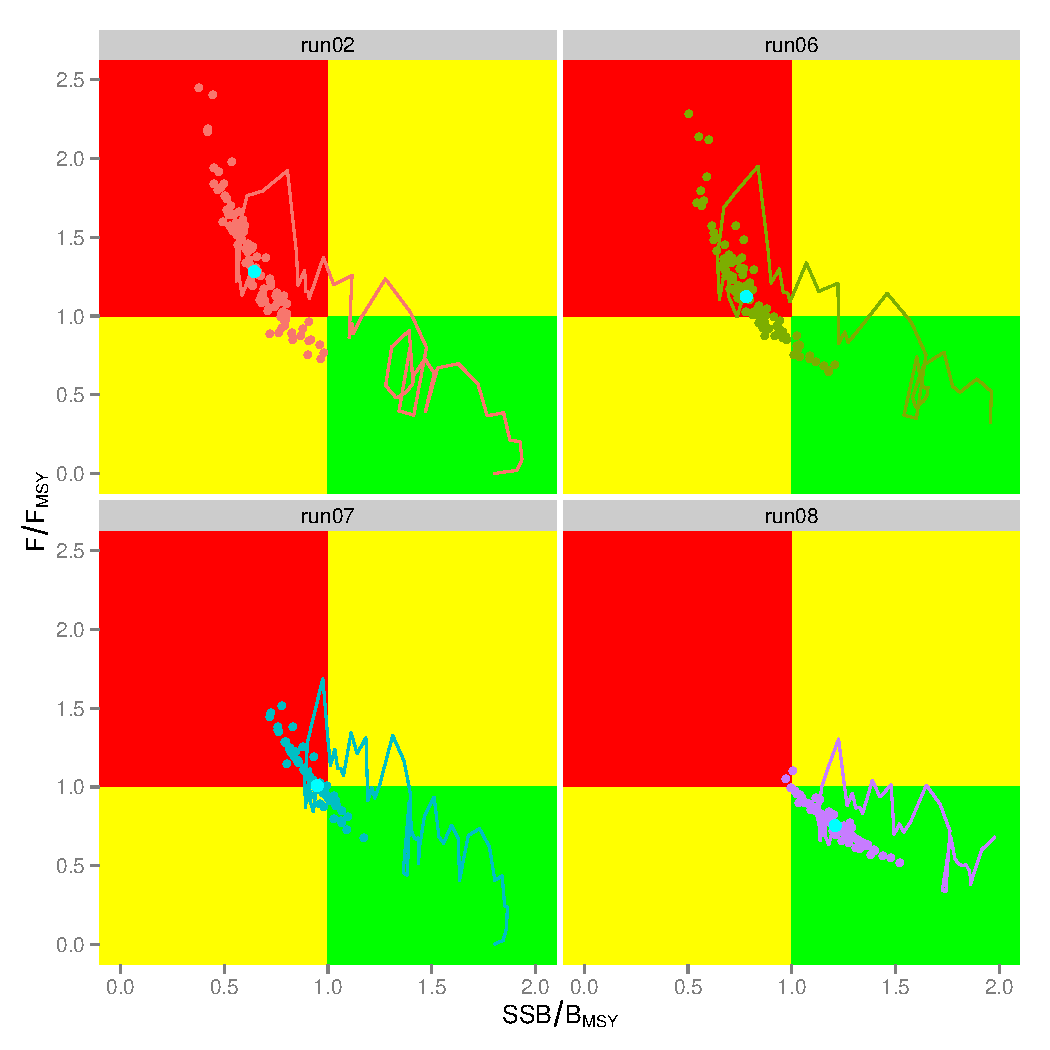
\includegraphics{kobe-018}
\caption{Phase plot of fishng mortality and stock status reletive to $F_{MSY}$ and  $B_{MSY}$, large point and lines are the medians
from the assessment and the panels correspond to  each run.}
\end{center}\end{figure}

The phase plots show the cross correlations between stock and harvest, but many points overlay each other so it is hard
to determine the actual probabilities or densities. To overcome this difficulty contours showing the bivariate probabilities 
can be plotted using \code{kobeP} e.g.

\begin{Schunk}
\begin{Sinput}
> kp2 = kp + geom_path(aes(x,y,group=level),colour="blue",
+                     data=ddply(subset(sims,year==2010 & TAC==15000),.(Run), 
+                                function(pts) kobeProb(pts$stock,pts$harvest,prob=c(0.7,.5,.25)))) +
+                     facet_wrap(~Run) + 
+                     theme(legend.position = "none")
\end{Sinput}
\end{Schunk}

\begin{figure}\begin{center}
\begin{Schunk}
\begin{Sinput}
> print(kp2)
\end{Sinput}
\end{Schunk}
\includegraphics{kobe-020}
\caption{Phase plot of fishng mortality and stock status reletive to $F_{MSY}$ and  $B_{MSY}$, large point and lines are the medians
from the assessment and the panels correspond to  each run.}
\end{center}\end{figure}

\clearpage
Alternatively the marginal densities can be plotted e.g.

\begin{figure}\begin{center}
\begin{Schunk}
\begin{Sinput}
> pts =subset(sims, year==2010 & TAC==15000)
> # stock density plot
> ggplot(pts) + 
+   geom_density(aes(x=stock, y= ..count.., group=Run, fill=Run, alpha=0.4))
\end{Sinput}
\end{Schunk}
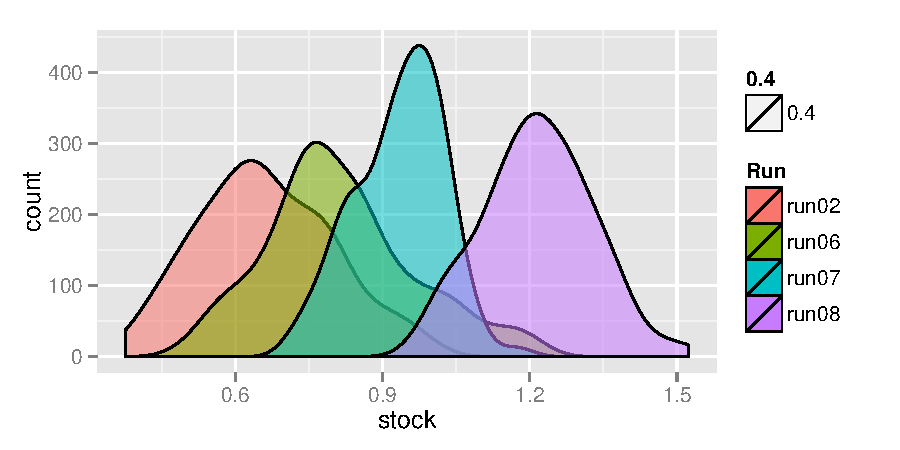
\includegraphics{kobe-021}
\end{center}\end{figure}

These show the values overlayed and so do not show the combined density. The same data can be also plotted by stacking them on top
of one another e.g.

\begin{figure}\begin{center}
\begin{Schunk}
\begin{Sinput}
> ggplot(pts) + 
+   geom_density(aes(x=stock, y=..count.., group=Run, fill=Run), 
+                         fill="grey", col=grey(.9), position = "stack") 
\end{Sinput}
\end{Schunk}
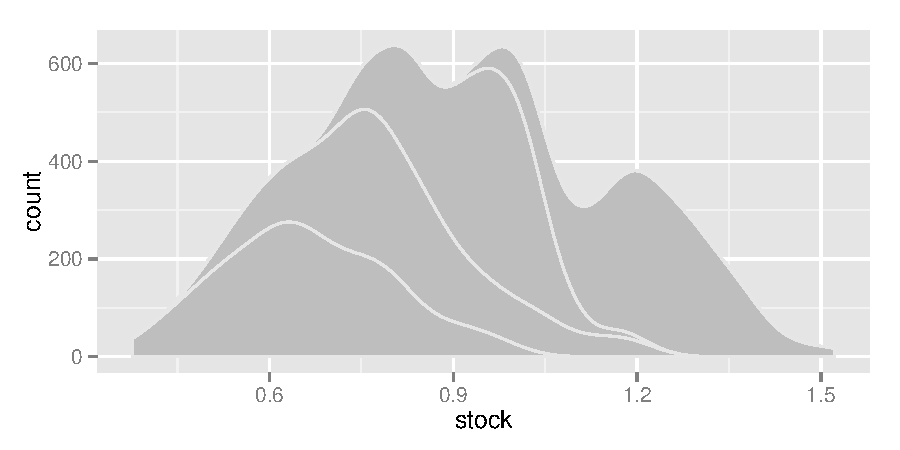
\includegraphics{kobe-022}
\end{center}\end{figure}

The phase and marginal density plots can be combined using \code{kobePhasemar} e.g.

\begin{figure}\begin{center}
\begin{Schunk}
\begin{Sinput}
> ### Bespoke Stuff ###
> print(kobePhaseMar(transform(pts,group=Run)))          
\end{Sinput}
\begin{Soutput}
$harvest

$stock

$phase
\end{Soutput}
\end{Schunk}
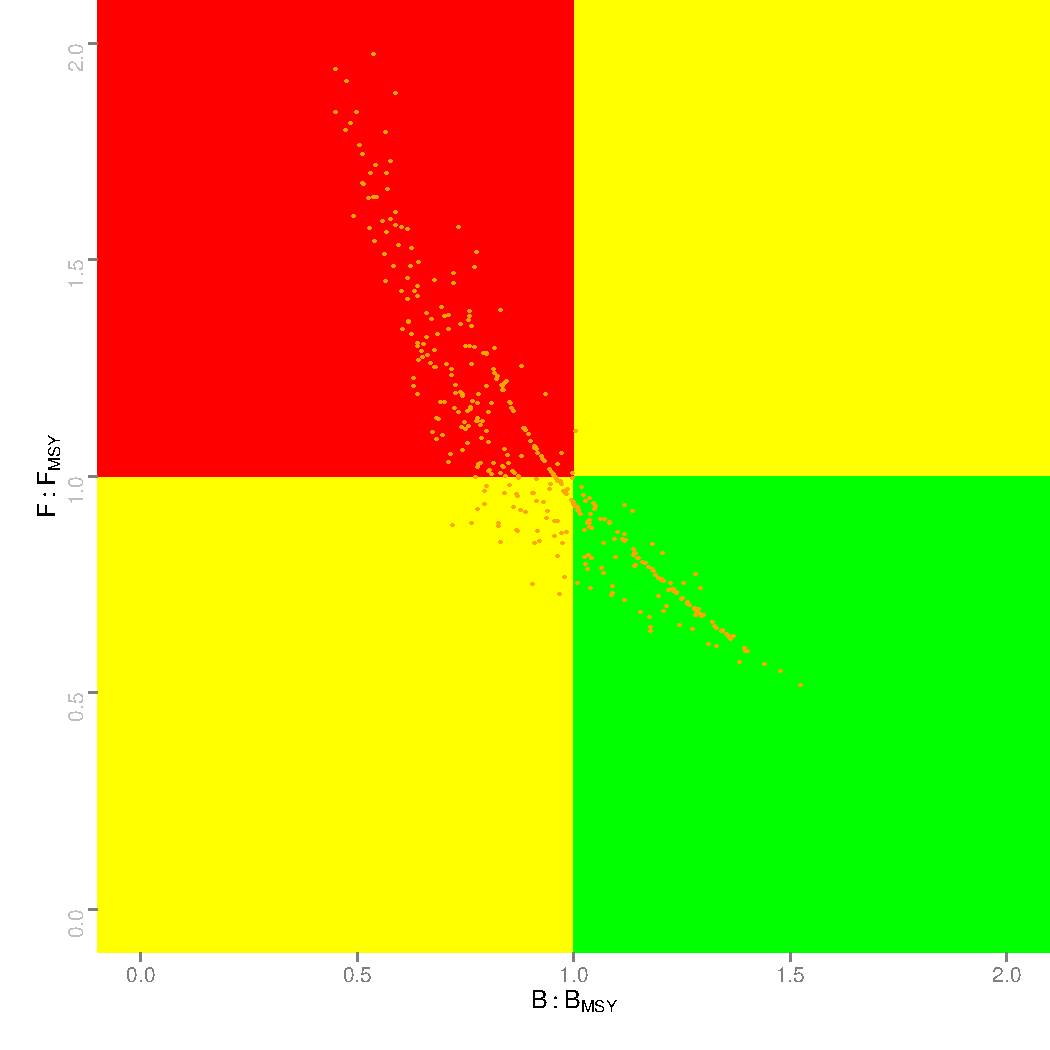
\includegraphics{kobe-023}
\end{center}\end{figure}

\clearpage

\subsubsection{Pie Charts}

Although pie charts have their critics ...

\begin{figure}\begin{center}
\begin{Schunk}
\begin{Sinput}
> ### Pies ###
> pie.dat=ddply(subset(sims,year==2010 & TAC==15000),.(Run),kobeSmry,o=T)
> pie.dat=ddply(melt(pie.dat,id.vars="Run"),.(Run,variable), 
+               function(x) data.frame(value=mean(x$value)))
> ## pie charts
> ggplot(subset(pie.dat,value>0), aes(x =factor(1), y=value, fill = variable)) + 
+   geom_bar(width = 1) + 
+   coord_polar(theta="y") +
+   labs(fill='Kobe Quadrant') + xlab('') + ylab('')       +
+   scale_fill_manual(values=c("red","green","yellow"))    + 
+   facet_wrap(~Run)                                       + 
+   scale_x_discrete(breaks=NULL)                          +
+   scale_y_continuous(breaks=NULL) 
\end{Sinput}
\end{Schunk}
\includegraphics{kobe-024}
\end{center}\end{figure}


\clearpage
\subsubsection{Kobe II Strategy Matrix}

\begin{figure}\begin{center}
\begin{Schunk}
\begin{Sinput}
> kobe2012=subset(sims,year %in% 2013:2022)
> pdat=subset(ddply(kobe2012,.(year,TAC),kobeSmry),
+             select=c(year,TAC,green,underFished,underFishing))
> pdat=melt(pdat,id.vars=c("year","TAC"))
> pdat=ddply(pdat, .(variable), function(x) kobeInterp(data.frame(x$year,x$TAC,x$value)))
> col.=c(colorRampPalette(c("red4","red"))(12),
+        colorRampPalette(c("yellowgreen","darkgreen"))(8))
> k2p = ggplot(aes(x=x,y=y,z=w),data=pdat)                 +
+            geom_tile(aes(x,y,fill=z))                    +
+            scale_fill_manual(values=col.,guide="none")   +
+            stat_contour(aes(colour= ..level..),size=1.2,  
+                             breaks=c(0.6,0.7,0.8,0.9))   +
+            scale_colour_gradient(low="grey", high="black", 
+                                  breaks=c(0.6,0.7,0.8,0.9),
+                                   labels=c(0.6,0.7,0.8,0.9),limits=c(0.6,1))    +
+            facet_wrap(~variable,ncol=1)                       +
+            xlab("Year")+ylab("TAC") 
> k2p
\end{Sinput}
\end{Schunk}
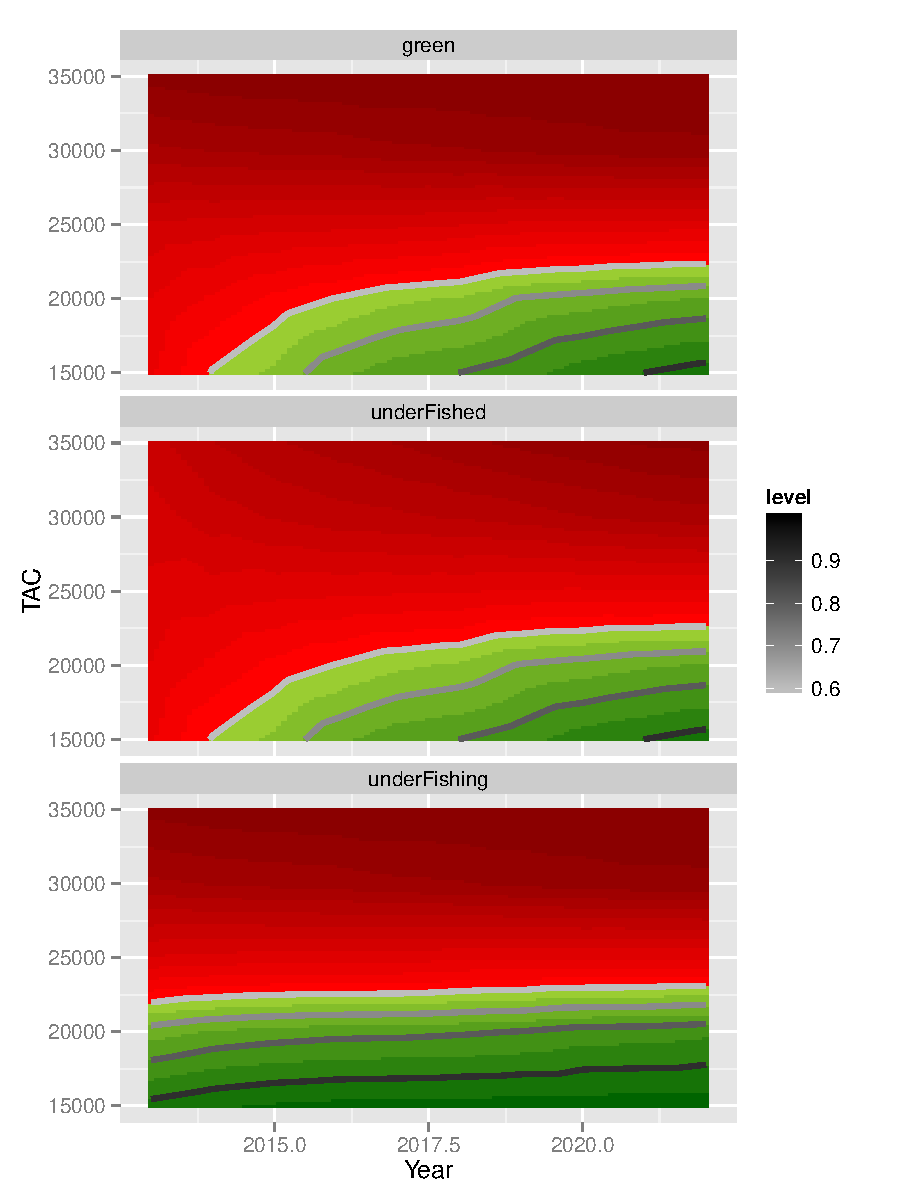
\includegraphics{kobe-025}
\end{center}\end{figure}


\clearpage
\section{Tabulation}

\subsection{Kobe II Strategy Matrix}

Three Kobe matrices Tables~\ref{tab:k2sm1}, \ref{tab:k2sm3} and \ref{tab:k2sm3} summarise the probabilities (by the ranges 
of 50-59 \%, 60- 69 \%, 70-79 \%, 80-89 \% and greater or equal to 90 \%) for different levels of catch across multiple years of 

\begin{itemize}
 \item  Biomass or SSB being greater than $B_{MSY}$ ;
 \item  Fishing Mortality or Harvest Rate being less than $F_{MSY}$; and 
 \item  the combined probability of Biomass or SSB being greater than $B_{MSY}$ and Fishing Mortality or Harvest Rate being less than $F_{MSY}$ 
\end{itemize}


\begin{Schunk}
\begin{Sinput}
> t.=ddply(subset(sims,year %in% 2013:2022),.(year,TAC),  kobeSmry)
> k2smTab=list()
> k2smTab[[1]]=cast(subset(t., year %in% 2013:2022),TAC~year,value="underFishing")
> k2smTab[[2]]=cast(subset(t., year %in% 2013:2022),TAC~year,value="underFished")
> k2smTab[[3]]=cast(subset(t., year %in% 2013:2022),TAC~year,value="green")
\end{Sinput}
\end{Schunk}


\end{document}

%<<results=hide, quiet=TRUE, echo=FALSE>>=
%# Making sure we can source code from github
%source("http://www.r-statistics.com/wp-content/uploads/2012/01/source_https.r.txt")
 
%# Reading in the function for using tabular on a cast_df object:
%source_https("https://raw.github.com/talgalili/R-code-snippets/master/tabular.cast_df.r")
%@ 


%<<results=tex,quite=TRUE,echo=FALSE>>=
%latex(tabular.cast_df(k2smTab[[1]]),caption="Kobe II Strategy Matrix, $P(F\\leq F_{MSY})$.")
%@ 


%<<echo=TRUE,quite=TRUE,echo=FALSE>>=
%library(tables)
%latex(tabular.cast_df(k2smTab[[3]]))
%@ 
%\caption{Kobe II Strategy Matrix, $P(SSB\\geq B_{MSY})$).}
                  
%<<results=tex,quite=TRUE,echo=FALSE>>=
%latex(tabular.cast_df(k2smTab[[3]]))
%@ 
%\caption{Kobe II Strategy Matrix, $P(F\\leq F_{MSY})$ and $P(SSB\\geq B_{MSY})$.}

